\chapter{Implementace}\label{implementation}

V této kapitole se budu věnovat převážně některým obecným součástem aplikace a jak jsem došel k jejich výsledné podobě. Obsahem \emph{není} popis realizace funkčních požadavků aplikace, přestože jsem jejich implementaci strávil nezanedbatelné množství času. Tento popis je již totiž dostupný ve formě analýzy a návrhu, kterým odpovídá.\\

%%%%%%%%%%%%%%%%%%%%%%%%%%%%%%%%%%%%%%%%%%%%%%%%%%%%%%%%%%%%%%%%%%%%%%%%%%%%%%%%
%%%%%%%%%%%%%%%%%%%%%%%%%%%%%%%%%%%%%%%%%%%%%%%%%%%%%%%%%%%%%%%%%%%%%%%%%%%%%%%%
%%%%%%%%%%%%%%%%%%%%%%%%%%%%%%%%%%%%%%%%%%%%%%%%%%%%%%%%%%%%%%%%%%%%%%%%%%%%%%%%
%%%%%%%%%%%%%%%%%%%%%%%%%%%%%%%%%%%%%%%%%%%%%%%%%%%%%%%%%%%%%%%%%%%%%%%%%%%%%%%%

\section{Nízkoúrovňové vývojové nástroje}

\subsection{Webpack}

Webpack \cite{webpack} je software, který zpracovává součásti webových aplikací a tvoří z nich balíčky vhodné pro webové prohlížeče. Primárně je zaměřen na Javascript, ale dokáže zpracovávat i řadu dalších formátů, přes styly v css, sass či stylus, obrázky v png, jpg, svg, ale také konfigurace v json, yaml a dalších.\\
Hlavním důvodem, proč používat Webpack, je možnost rozdělování kódu do jednotlivých souborů. Při programování je pohodlné mít oddělené ucelené komponenty, různé konfigurační soubory apod. Výstupem webpacku jsou poté typicky pouze čtyři soubory: dva obsahující logiku aplikace (.js) a dva pro stylování (.css), přičemž logika i styly jsou rozděleny na samotnou aplikaci - kód programátora, a kód třetích stran - tzv. \code{vendor}.

\paragraph{Použití loaderů.} Další příležitost k použití webpacku přichází ve chvíli, kdy chceme v projektu mít kód, který není v cílovém prohlížeči podporován. Tím může být například SASS, nebo třeba i moderní syntaxe Javascriptu řídící se standardem ES6 či novějším. S pomocí Webpacku lze nastavit, aby se při zpracování některých assetů použil \emph{loader}, který například převede SASS na CSS, konstrukce ES6 na ES5 apod. \cite{webpack-ackee}.

\paragraph{Webpack ve spolupráci s Vue.js.} Konfigurace webpacku může být pro neznalého uživatele až příliš obsáhlá a může být jednoduché v ní udělat chybu, kvůli které bude například výsledný build aplikace neoptimalizovaný a tudíž pomalý. Vývojáři Vue tento problém mitigovali tak, že celá optimalizovaná konfigurace webpacku je součástí \code{vue-cli}, což znamená, že stačí mít v projektu jako závislosti právě tento npm modul, a pokud nejsou vyžadovány žádné pokročilé funkce, funguje vše \emph{automagicky}\footnote{Nejedná se o překlep, jde o spojení slov automaticky a magicky}. Pro účely porovnání jsem se podíval, jak dlouhá je konfigurace webpacku, kterou má Vue automaticky v sobě - jedná se o \emph{1490 řádků kódu}.

%%%%%%%%%%%%%%%%%%%%%%%%%%%%%%%%%%%%%%%%
%%%%%%%%%%%%%%%%%%%%%%%%%%%%%%%%%%%%%%%%

\subsection{Vue-UI}

V předchozím paragrafu jsem popisoval výhodu použití Vue-CLI, ke kterému je ale vhodné říci i několik dalších slov, jelikož se jedná o velmi prakticky nástroj, usnadňující mnoho běžných požadavků na správu projektu.\\
Zaměřit bych se chtěl především na možnost spuštění grafického prostředí, pomocí \code{vue ui} z terminálu, což si vytvoří vlastní webový server a na adrese \code{localhost:8000} spustí grafickou správu projektu. Ta obsahuje následující možnosti:
\begin{itemize}
    \item \emph{přehled projektů}, který nabízí rychlou kontrolu dostupných aktualizací použitých balíčků, kontrolu bezpečnostních mezer nebo RSS čtečku novinek od Vue komunity,
    \item \emph{instalované pluginy}, což jsou běžné npm balíčky, ke kterým je ale možné přidat další konfiguraci. Jedný se například o pluginy pro samotné \code{vue-cli}, \code{eslint} nebo třeba knihovnu \code{vuetify}, která poskytuje grafické komponenty, a pomocí tohoto pluginu vkládá do výsledného buildu pouze ty, které jsou skutečně v aplikaci používány.
    \item \emph{instalované závislosti}, u kterých je možné jednoduše hromadně aktualizovat na nové verze, zobrazovat, jakou verzi používáme a jaká je nejnovější, nebo přes jednotné hledání instalovat nové závislosti,
    \item \emph{úlohy spouštěné nad kódem aplikace}, asi nejpraktičtější součást Vue-UI, ze které je možné spouštět lokální dev-server ale také build pro produkci. Největší výhodou spouštění těchto úloh z UI je ta, že po skončení úlohy jsou zde dostupné bohaté informace o velikosti výsledných souborů a přehled, jak velká je která závislost. Jako příklad uvedu dále optimalizaci velikosti překladů.
\end{itemize}

\paragraph{Optimalizace velikosti aplikace odebráním zbytečných překladů.} Jednou ze závislostí, kterou v projektu používám, je knihovna \emph{moment} \cite{momentjs}, která se stará o parsování a zobrazování datumů a časů, a jejíž součástí jsou i překlady do 127 jazyků. Jeden soubor s jazykem má sice \uv{pouze} 172 řádků kódu, ale při vzájemném pronásobení to už je \emph{21844 řádků}. Není tak divu, že při analýze velikostu výsledných souborů pomocí Vue-UI jsem odhalil, že tyto překlady zabírají téměř \emph{15\% celé velikosti} souboru s kódem třetích stran (\code{vendor}), jak je znázorněno na obrázku \ref{picture:cli:analyze}.

\begin{figure}[]
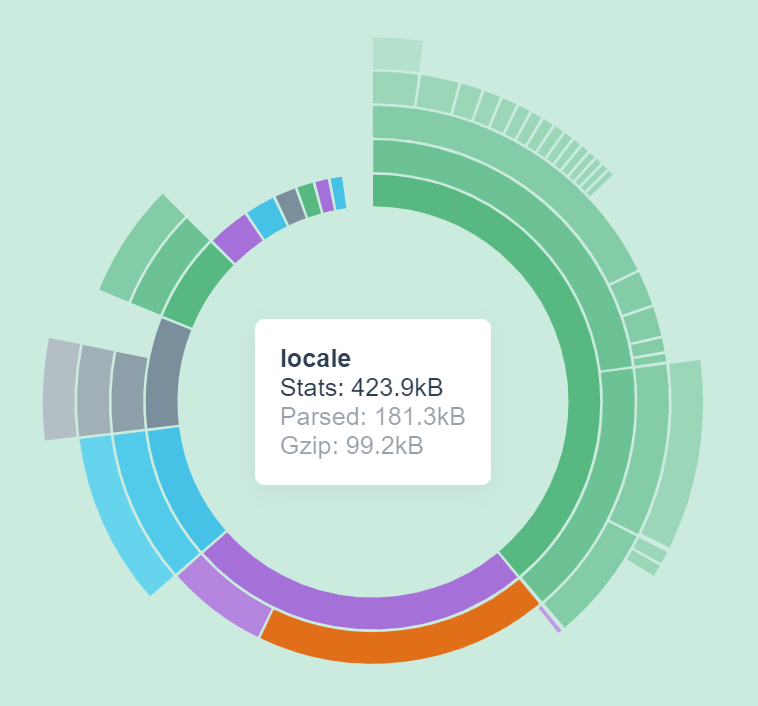
\includegraphics[width=0.7\textwidth]{../png/cli/analyze-moment.png}
\caption[Analýza velikosti výsledné aplikace: překlady moment.js]{Analýza velikosti výsledné aplikace: překlady moment.js (na obrázku popsáno jako locale a označeno oranžově) zabírají velké procento z celkové velikosti souboru.} \label{picture:cli:analyze}
\end{figure}

Našel jsem si tedy řešení spočívající v přidání jednoho řádku konfigurace \cite{momentjs-ignore-locale}, jehož cílem je nezahrnovat do výsledného buildu ty jazyky, které nepoužívám (což jsou všechny, kromě češtiny a angličtiny). Výsledek je takový, že nyní překlady nezabírají \emph{ani jedno celé procento}.

%%%%%%%%%%%%%%%%%%%%%%%%%%%%%%%%%%%%%%%%
%%%%%%%%%%%%%%%%%%%%%%%%%%%%%%%%%%%%%%%%

\subsection{Proměnné prostředí}

TODO

%%%%%%%%%%%%%%%%%%%%%%%%%%%%%%%%%%%%%%%%%%%%%%%%%%%%%%%%%%%%%%%%%%%%%%%%%%%%%%%%
%%%%%%%%%%%%%%%%%%%%%%%%%%%%%%%%%%%%%%%%%%%%%%%%%%%%%%%%%%%%%%%%%%%%%%%%%%%%%%%%
%%%%%%%%%%%%%%%%%%%%%%%%%%%%%%%%%%%%%%%%%%%%%%%%%%%%%%%%%%%%%%%%%%%%%%%%%%%%%%%%
%%%%%%%%%%%%%%%%%%%%%%%%%%%%%%%%%%%%%%%%%%%%%%%%%%%%%%%%%%%%%%%%%%%%%%%%%%%%%%%%

\section{Router}

Jednou z prvních komponent, kterou jsem k čistému Vue.js přidal, byl oficiální Vue Router \cite{vue-router}. Koncept routeru je dobře znám z jakékoliv jiné aplikace, která nějak pracuje s prohlížečem uživatele.\\
Rozdíl Vue.js routeru oproti tomu, který je používán třeba v PHP, spočívá v dynamičnosti celého Javascriptového frameworku: oproti standardním webovým stránkám, kde přesměrování na novou adresu skutečně vyvolá požadavek na server, který odpoví obsahem stránky na dané URL (diagram \ref{picture:route:http}), zde se vše děje dynamicky přímo na klientském zařízení, obsah je vyměněn pomocí Javascriptu a hodnota adresního řádku se změní pouze \uv{pro efekt} - tj. aby uživatel věděl, kde se nachází, a aby mohl adresu zkopírovat a sdílet. Samozřejmě i zde většinou dochází k načítání dat nově otevřené stránky, ale vše je typicky asynchronní - stránka se změní ihned a teprve poté jsou do ní doplněna data - viz diagram \ref{picture:route:vue}.

\begin{figure}[]
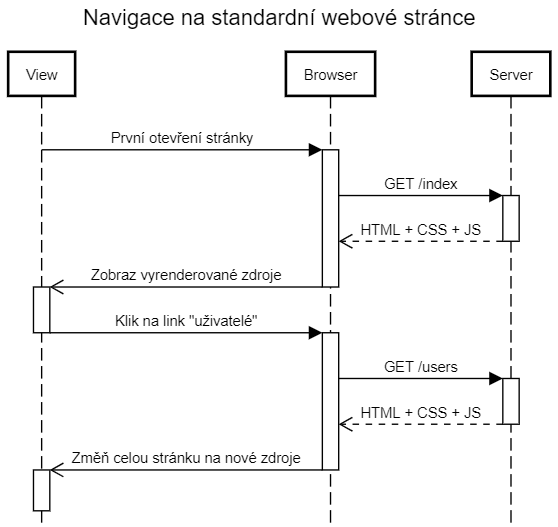
\includegraphics[width=0.7\textwidth]{../png/diagrams/sequence-http-navigate.png}
\caption[Navigace na standardní webové stránce]{Navigace na standardní webové stránce: Pro každý link existuje cesta na serveru, který odpovídá kompletním obsahem této stránky.} \label{picture:route:http}
\end{figure}

\begin{figure}[]
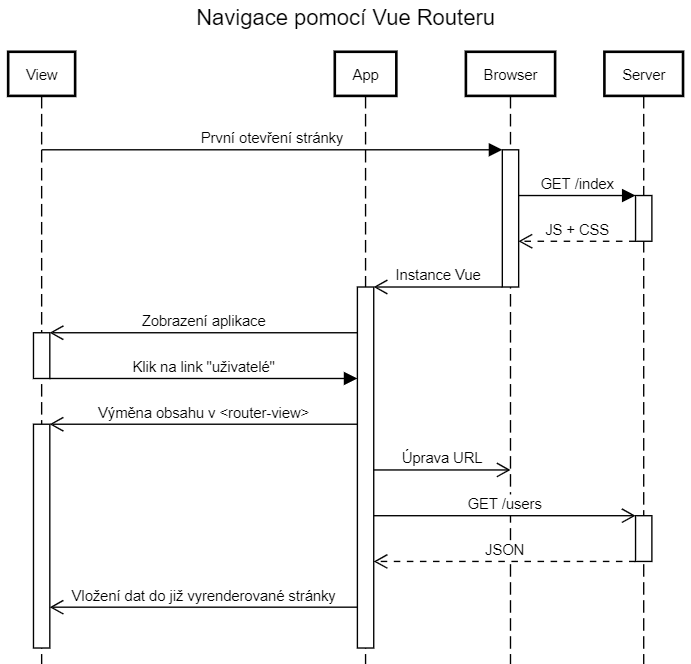
\includegraphics[width=0.9\textwidth]{../png/diagrams/sequence-vue-router.png}
\caption[Navigace v aplikaci pomocí Vue Router]{Navigace v aplikaci pomocí Vue Router: Kompletní obsah aplikace se ze serveru stáhne pouze při prvním přístupu, navigaci v aplikaci řeší Vue Router přímo na klientu a od serveru či jiného API vyžaduje pouze konkrétní data, která v aplikaci zobrazuje.} \label{picture:route:vue}
\end{figure}

% title Navigace na standardní webové stránce

% View->Browser:První otevření stránky
% activate Browser
% Browser->Server:GET /index
% activate Server
% Server-->>Browser:HTML + CSS + JS
% deactivate Server
% Browser->>View:Zobraz vyrenderované zdroje
% deactivate Browser
% activate View


% View->Browser:Klik na link "uživatelé"
% deactivate View
% activate Browser
% Browser->Server:GET /users
% activate Server
% Server-->>Browser:HTML + CSS + JS
% deactivate Server
% Browser->>View:Změň celou stránku na nové zdroje
% deactivate Browser
% activate View


% title Navigace pomocí Vue Routeru
% 
% participant View
% participant App
% participant Browser
% participant Server
% 
% View->Browser:První otevření stránky
% activate Browser
% Browser->Server:GET /index
% activate Server
% Server-->>Browser:JS + CSS
% deactivate Server
% Browser->>App:Instance Vue
% deactivate Browser
% activate App
% App->>View:Zobrazení aplikace
% activate View
% 
% 
% View->App:Klik na link "uživatelé"
% deactivate View
% App->>View:Výměna obsahu v <router-view>
% activate View
% App->>Browser:Úprava URL
% App->>Server:GET /users
% activate Server
% Server-->>App:JSON
% deactivate Server
% App->>View:Vložení dat do již vyrenderované stránky
% 

\paragraph{Titulky stránek.} Lehce matoucí může u tohoto \emph{frontendového routování} být nastavování titulků stránek, tedy \code{<title>} tagů v HTML. Celá aplikace má totiž stále pouze jeden \code{<title>} zapsaný v souboru \code{index.html}, který se sám o sobě při navigaci za pomocí routeru vůbec nemění. K vyřešení tohoto problému sice ve Vue Routeru neexistuje nativní podpora, ale řešení je opravdu snadné - je popsáno v jednom z \emph{issues} v repozitáři na GitHubu \cite{vue-router-title} a spočívá v doplnění titulků do \code{meta} atributů cest, viz ukázka kódu \ref{code:vue-router-title1}, a dále úpravě samotné instance routeru, viz ukázka kódu \ref{code:vue-router-title2}.

\begin{listing}[]
\begin{minted}[linenos,frame=lines]{javascript}
{
    path: '/',
    component: Homepage,
    meta: {
        title: 'Swordfish'
    }
}
\end{minted}
\caption{Nastavování titulků stránek pomocí Vue routeru - úprava definic} \label{code:vue-router-title1}
\end{listing}

\begin{listing}[]
    \begin{minted}[linenos,frame=lines]{javascript}
router.beforeEach((to, from, next) => {
    document.title = to.meta.title;
    next();
})
\end{minted}
\caption{Nastavování titulků stránek pomocí Vue routeru - úprava instance routeru} \label{code:vue-router-title2}
\end{listing}

Toto nastavování titulků stránek jsem nakonec ještě více upravil po svém, jelikož jsem chtěl mít v titulcích i konkrétní hodnoty, které se zobrazují na dané stránce - například při úpravě skladu \emph{Centrální sklad Praha} nechci mít v titulku \uv{Úprava skladu}, ale \uv{Úprava skladu 'Centrální sklad Praha'}. Jelikož jsou ale tyto informace načítány dynamicky až po vstupu na danou stránku (URL stránky může být například \code{/stocks/12/edit} - z té to tedy vyčíst nelze), je nutné i titulek nastavovat dynamicky. Zachoval jsem tedy jako výchozí hodnotu titulku stránky ten, který je nastaven přímo v definici cesty v routeru (ukázka kódu \ref{code:vue-router-title1}), avšak zevnitř komponenty je možné pomocí jednotné funkce titulek obohatit dalšími informacemi - jako například názvem upravované položky.

\paragraph{Drobečková navigace.} Další úpravou routeru, kterou jsem do jisté míry realizoval po svém, je generování drobečkové navigace. Vue Router ve spojení s Vuetify nemají nativní podporu pro zjišťování rodičovských stránek, a tak jsem si lehkou úpravou a vlastní komponentou pro vykreslování \emph{Breadcrumbs} toto zautomatizoval:\\
Každá definovaná routa má nastaveného rodiče, ke kterému poskytuje \emph{getter}. Ve vykreslování drobečkové navigace se poté na aktuální routě zjišťují rekurzivně její rodiče, a včetně jejich parametrů se z nich zpětně tvoří celý strom navigace.\\
Co se na první pohled může zdát jednoduché, se zkomplikuje ve chvíli, kdy chceme mít v cestě parametrizovanou stránku.\\
Například v URL \code{/stocks/1/locations/12/update} je potřeba v definici routy nahradit všechny identifikátory jejich reálnými hodnotami, které ale naštěstí Vue Router poskytuje i během runtime. Funkce pro vytvoření jednoho odkazu, ze kterých se skládá drobečková navigace, je znázorněna v ukázce kódu \ref{code:router:buildPath} - jejími argumenty jsou definice cesty v routě a objekt s aktuálními hodnotami parametrů.

\begin{listing}[H]
    \begin{minted}[linenos,frame=lines]{javascript}
function buildPath(pathWithPlaceholders, parameters) {
    let routePath = pathWithPlaceholders.replace(/\([^/]+\)/g, '');
    const matches = routePath.match(/(:[a-zA-Z]+\/)|(:[a-zA-Z]+$)/g);
    if (matches !== null) {
        for (const match of matches) {
            const matchParam = match.replace(/\//, '').replace(/:/, '');
            routePath = routePath
                        .replace(match, parameters[matchParam] + '/');
        }
    }
    return routePath;
}
\end{minted}
\caption[Automatické generování drobečkové navigace]{Automatické generování drobečkové navigace z definic Vue Routeru, včetně podpory parametrizovaných zanořených cest} \label{code:router:buildPath}
\end{listing}

%%%%%%%%%%%%%%%%%%%%%%%%%%%%%%%%%%%%%%%%%%%%%%%%%%%%%%%%%%%%%%%%%%%%%%%%%%%%%%%%
%%%%%%%%%%%%%%%%%%%%%%%%%%%%%%%%%%%%%%%%%%%%%%%%%%%%%%%%%%%%%%%%%%%%%%%%%%%%%%%%
%%%%%%%%%%%%%%%%%%%%%%%%%%%%%%%%%%%%%%%%%%%%%%%%%%%%%%%%%%%%%%%%%%%%%%%%%%%%%%%%
%%%%%%%%%%%%%%%%%%%%%%%%%%%%%%%%%%%%%%%%%%%%%%%%%%%%%%%%%%%%%%%%%%%%%%%%%%%%%%%%

\section{Plnohodnotná webová aplikace}

V kapitole \ref{technology} jsem zmiňoval, že skladník bude aplikaci používat z nativní Android aplikace, která bude obalovat WebView, a vedoucí skladu si aplikaci otevře v běžném browseru - pro obě použití by níže popisovaná konfigurace nebyla potřeba, avšak pokud by někdo nepotřeboval čtečku čárových kódu - což je jediný důvod, proč skladníci používají jako základ nativní Android aplikaci, je možné si otevřít na mobilu běžnou stránku a použít volbu \uv{Přidat na plochu}. Tím vznikne zástupce, který zobrazuje \emph{favicon} webové stránky a po jehož otevření se opět otevře běžný webový prohlížeč.\\
Pokud je však na stránce definovaný \code{manifest.json} pro webové aplikace, může se po otevření tohoto zástupce otevřít stránka v režimu celé obrazovky, a to případně i se skrytými ovládacími prvky - vše tak vypadá, jako kdyby se jednalo o nativní nainstalovanou aplikaci. Základní konfigurace tohoto manifestu je vidět v ukázce kódu \ref{code:webapp-manifest}.

\begin{listing}[H]
\begin{minted}[linenos,frame=lines]{json}
{
  "name": "Swordfish",
  "icons": [
    {
      "src": "favicon/swordfish-192x192.png",
      "sizes": "192x192",
      "type": "image/png"
    },
    {
      "src": "favicon/swordfish-512x512.png",
      "sizes": "512x512",
      "type": "image/png"
    }
  ],
  "start_url": "/",
  "display": "standalone",
  "orientation": "portrait",
  "background_color": "#009688"
}

\end{minted}
\caption{Manifest pro webové aplikace} \label{code:webapp-manifest}
\end{listing}

Tento soubor je vlastně také první krok k vytvoření PWA - Progresivní webové aplikace, což znamená takové webové aplikace, která do jisté míry může fungovat i bez připojení k internetu. Využívá k tomu Service Worker API \cite{service-worker-api}, jehož specifikace je v době psaní tohoto textu stále ve stavu návrhu, přestože vzniká již od května roku 2014 \cite{service-worker-first}.\\
I přes nedokončenou speficikaci se již PWA běžně používají a i ve skladové aplikaci by bylo vhodné toto API využít, to již ale není předmětém této práce a proto jej v tuto chvíli dále nerozvádím.

%%%%%%%%%%%%%%%%%%%%%%%%%%%%%%%%%%%%%%%%%%%%%%%%%%%%%%%%%%%%%%%%%%%%%%%%%%%%%%%%
%%%%%%%%%%%%%%%%%%%%%%%%%%%%%%%%%%%%%%%%%%%%%%%%%%%%%%%%%%%%%%%%%%%%%%%%%%%%%%%%
%%%%%%%%%%%%%%%%%%%%%%%%%%%%%%%%%%%%%%%%%%%%%%%%%%%%%%%%%%%%%%%%%%%%%%%%%%%%%%%%
%%%%%%%%%%%%%%%%%%%%%%%%%%%%%%%%%%%%%%%%%%%%%%%%%%%%%%%%%%%%%%%%%%%%%%%%%%%%%%%%

\section{Překlady}

Novou aplikaci je dnes vhodné hned od počátku psát jako \emph{multijazyčnou} - jako základ tedy například v češtině a angličtině.\\
Pro překlady Vue.js aplikací je vhodné použít knihovnu \code{vue-i18n}\footnote{název je zkratka slova \emph{internationalization} - číslovka 18 značí počet přeskočených znaků} \cite{vue-i18n}, jejíž použití je obdobné, jako známe z jiných jazyků. Zatímco například v PHP se často překlady zapisují do \code{.yaml} nebo \code{.neon}, což jsou formáty, které sice umožňují například zanořování, ale s dalšími funkcemi už si často neporadí, zde se texty zapisují do běžného \code{.js} souboru (ukázka kódu \ref{code:i18n-def}), jehož výstupem je JSON. To znamená, že můžeme používat libovolné konstrukce Javascriptu, od standarního zápisu (klíč \code{close} ve zmiňované ukázce), přes spojování řetězců a používání konstant (podklíče \code{user}), po proměnné klíče (podklíče \code{orderState}), jejichž definice se doplní z číselníku načteného klidně i z jiného souboru. Kreativní autor překladů by jistě našel i prostor pro použití cyklů nebo funkcí, mně ale pro potřeby skladové aplikace stačily znázorněné možností.

\begin{listing}[h]
\begin{minted}[linenos,frame=lines]{js}
const user = "uživatele";

{
    close: "Zavřít",
    user: {
        create: "Vytvořit " + user,
        update: "Upravit " + user
    },
    orderState: {
        [OrderStateEnum.CREATED]: 'Vytvořená',
        [OrderStateEnum.SENT]: 'Odeslaná',
    }
}
\end{minted}
\caption[Definice překladů pro i18n]{Definice překladů pro i18n, včetně pokročilých funkcí jako například spojování řetězců nebo využítí číselníků.} \label{code:i18n-def}
\end{listing}

\paragraph{Překlady a uživatelská nápověda.} Jelikož výsledná aplikace obsahuje i stručnou nápovědu, která má zatím pouze textový obsah, využil jsem pro zápis jejího obsahu také formát, který používá \code{i18n} pro překlady. Tyto texty jsem ale neintegroval do seznamu obecných překladů v aplikaci, ale pracuji s nimi odděleně - pomocí vlastního řešení pro zobrazování nápovědy. Tím mohu všechny texty této \uv{sekce} načíst hromadně a umožnit v nich například vyhledávání, nebo je vkládám přímo k formulářovým atributům, které dokumentují.

%%%%%%%%%%%%%%%%%%%%%%%%%%%%%%%%%%%%%%%%%%%%%%%%%%%%%%%%%%%%%%%%%%%%%%%%%%%%%%%%
%%%%%%%%%%%%%%%%%%%%%%%%%%%%%%%%%%%%%%%%%%%%%%%%%%%%%%%%%%%%%%%%%%%%%%%%%%%%%%%%
%%%%%%%%%%%%%%%%%%%%%%%%%%%%%%%%%%%%%%%%%%%%%%%%%%%%%%%%%%%%%%%%%%%%%%%%%%%%%%%%
%%%%%%%%%%%%%%%%%%%%%%%%%%%%%%%%%%%%%%%%%%%%%%%%%%%%%%%%%%%%%%%%%%%%%%%%%%%%%%%%

\section{State management pattern}

TODO + moje persistentní řešení

Jako první se zde sluší říci, co to vlastně \emph{State management pattern} je. Ve Vue.js aplikaci máme typicky velké množství komponent, a ty mezi sebou často potřebují komunikovat. Pěkný příklad je například \emph{snackbar message}, někdy nazývaná také \emph{toast message} či jednoduše \emph{oznámení o provedení akce}. To je komponenta, která musí být dostupná z jakékoliv jiné komponenty systému a vždy se musí zobrazovat na stejném místě a stejně se chovat. Je tedy žádoucí zpřístupnit její \emph{stav} a to tak, aby se při změně stavu něco automaticky stalo, a aby změna stavu byla řízena jistými pravidly.

\paragraph{Vuex.} Vuex \cite{vuex} je knihovna, která implementuje \emph{State management pattern} pro Vue.js. Zařizuje jednotný přístup ke stavům komponent a umožňuje jejich řízené změny. Jeho použití v aplikaci skladového systému je vidět na ukázce kódu \ref{code:vuex-snack-def}, \ref{code:vuex-snack-snack} a \ref{code:vuex-snack-use}, kde řeší zobrazování \emph{snackbar message}.

\begin{listing}[h]
\begin{minted}[linenos,frame=lines]{js}
Vue.use(Vuex);

new Vue({
    store: new Vuex.Store({
        modules: {
            snackbar: {
                state: {
                    snack: ''
                },
                mutations: {
                    setSnack (state, snack) {
                        state.snack = snack
                    }
                },
            }
        }
    });
});
\end{minted}
\caption{Vuex pro snackbar-message: definice} \label{code:vuex-snack-def}
\end{listing}

\begin{listing}[h]
\begin{minted}[linenos,frame=lines]{js}
...
export default {
    name: "Snackbar",
    data: ...
    created: function () {
        this.$store.watch(state => state.snackbar.snack, () => {
            const msg = this.$store.state.snackbar.snack;
            if (msg !== '') {
                this.show = true;
                this.text = msg;
                this.$store.commit('setSnack', '');
            }
        })
    }
}
\end{minted}
\caption{Vuex pro snackbar-message: Snackbar komponenta} \label{code:vuex-snack-snack}
\end{listing}

\begin{listing}[h]
\begin{minted}[linenos,frame=lines]{js}
this.$store.commit('setSnack', '<message to display>');
\end{minted}
\caption{Vuex pro snackbar-message: použití z jiné komponenty} \label{code:vuex-snack-use}
\end{listing}

Kód z ukázky \ref{code:vuex-snack-use} se mi ovšem v průběhu psaní aplikace přestal líbit, neboť zobrazování těchto zpráv je velmi častá operace, a jeho vyvolání není v ukázce příliš jednoduché. Proto jsem si nastudoval Mixiny ve Vue.js \cite{vue-mixins} a vytvořil mixin, který zjednodušuje zasílání zpráv do Snackbaru. Použití v komponentě je znázorněné na ukázce kódu \ref{code:snack-mixin}. Kromě tohoto použití je sice navíc potřeba v komponentě nastavit, aby importovala a používala nově vytvořený mixin, který poskytuje právě metodu \code{snack()}, avšak, to lze vše provést během programování automaticky za pomoci IDE.

\begin{listing}[h]
\begin{minted}[linenos,frame=lines]{js}
this.snack('<message to display');
\end{minted}
\caption{Použití mixinu pro zjednodušení zasílání zpráv do Snackbaru} \label{code:snack-mixin}
\end{listing}

%%%%%%%%%%%%%%%%%%%%%%%%%%%%%%%%%%%%%%%%%%%%%%%%%%%%%%%%%%%%%%%%%%%%%%%%%%%%%%%%
%%%%%%%%%%%%%%%%%%%%%%%%%%%%%%%%%%%%%%%%%%%%%%%%%%%%%%%%%%%%%%%%%%%%%%%%%%%%%%%%
%%%%%%%%%%%%%%%%%%%%%%%%%%%%%%%%%%%%%%%%%%%%%%%%%%%%%%%%%%%%%%%%%%%%%%%%%%%%%%%%
%%%%%%%%%%%%%%%%%%%%%%%%%%%%%%%%%%%%%%%%%%%%%%%%%%%%%%%%%%%%%%%%%%%%%%%%%%%%%%%%

\section{Hlídání konektivity}

V moderních aplikacích, které veškerá data ukládají na API, je vhodné hlídat dostupnost tohoto API.\\
Prvním krokem k realizaci této funkce bylo zjistit stav připojení - tedy zda je aplikace online, nebo offline. Jako první jsem našel vlastnost prohlížeče \code{window.navigator.onLine} \cite{online}, která by přesně o tomto měla informovat a navíc poskytuje i možnosti poslouchat její změny pomocí běžných JS eventů.\\
Po hlubším prozkoumání TODO
TODO kontrola konektivity (proč nepoužívat browser properities, vlastní check, jeho náročnost na síť)

%%%%%%%%%%%%%%%%%%%%%%%%%%%%%%%%%%%%%%%%%%%%%%%%%%%%%%%%%%%%%%%%%%%%%%%%%%%%%%%%
%%%%%%%%%%%%%%%%%%%%%%%%%%%%%%%%%%%%%%%%%%%%%%%%%%%%%%%%%%%%%%%%%%%%%%%%%%%%%%%%
%%%%%%%%%%%%%%%%%%%%%%%%%%%%%%%%%%%%%%%%%%%%%%%%%%%%%%%%%%%%%%%%%%%%%%%%%%%%%%%%
%%%%%%%%%%%%%%%%%%%%%%%%%%%%%%%%%%%%%%%%%%%%%%%%%%%%%%%%%%%%%%%%%%%%%%%%%%%%%%%%

\section{Renderování formulářů} \label{implementation:formRender}

\paragraph{Anti-inspirace v jiném projektu.} Ještě před tím, než jsem začal tvořit formuláře ve své diplomové práci, jsem shodou okolností potřeboval upravit několik formulářů v jiné aplikaci, která funguje na podobných technologiích: backend je zcela oddělený a poskytuje REST API, frontend je poté napsán v Angularu. Při zjišťování, jak složitě se zde generují formuláře jsem ale zjistil, že pro svou práci chci rozhodně vymyslet lepší systém. Níže přikládám seznam, které věci je potřeba ve zmiňovaném projektu upravit, chce-li programátor přidat nový formulářový prvek:

\begin{enumerate}
    \item přidat atribut do modelové třídy,
    \item nakódovat HTML, které atribut vypisuje,
    \item přidat atribut do instance formuláře,
    \item nastavovat výchozí obsah formuláře při načtení existujících dat z API,
    \item nastavovat nový obsah modelu při ukládání nových dat na API,
    \item nakódovat HTML, které umožňuje atribut měnit - tj. formulářový vstup.
\end{enumerate}

Celkem se tedy jedná o šest míst, kam je potřeba nový atribut zanést. Zde je ovšem na místě upozornit, že se rozhodně nejedná o problém Angularu, a že ve Vue.js není vše automaticky jednodušší - postup, jak jsem tento počet redukoval, by měl být použitelný v jakémkoliv Javascriptovém frameworku, a s většími úpravami pravděpodobně i v jiných jazycích.\\

\paragraph{Nový návrh renderování formulářů.} Co se mi zejména ve výše zmiňovaném řešení nelíbilo, byl fakt, že \emph{modelová třída} a \emph{instance formuláře} měly totožné atributy, tudíž se vůbec nemusí nastavovat jedna po druhé, ale můžeme použít například \code{Object.assign()} \cite{mdn-object-assign} pro nakopírování hodnot jednoho objektu do druhého. \emph{(Tato metoda sice není podporována v Android WebView, avšak napsat její ruční alternativu je triviální záležitost)}. Tím dokážeme odbourat nutnost nastavování konkrétních klíčů mezi instancí formuláře a modelovou třídou - tedy položky 4. a 5. výše uvedeného seznamu.\\
Nutnost položky č. 2 - vykreslování v HTML - jsem tušil už od začátku. Tomuto je spíše kontraproduktivní se vyhýbat, neboť typicky každý atribut chceme vypsat nějak jinak, celá stránka je nějak strukturována apod. - tuto položku jsem tedy ponechal a smířil se s tím, že se bude u výpisu formulářů vždy kódovat ručně.\\
Stále ale ještě máme nutnost nastavit atribut v modelové třídě, v instanci formuláře a formulář nějak vykreslovat - tedy na třech různých místech: dvakrát v Typescriptu a jedenkrát v HTML. Má představa o jednoduše konfigurovatelném formuláři se ubírala směrem k vytvoření pouze jednoho konfiguračního souboru, odkud by se všechny tyto 3 věci generovaly, což se mi nakonec podařilo, a seznam jsem tedy stáhl na:

\begin{enumerate}
    \item nastavit atribut v konfiguračním souboru,
    \item nakódovat HTML, které atribut vypisuje.
\end{enumerate}

Důležité je zde zdůraznit, že jsem odebral i nutnost vytvořit HTML kód formuláře: pokud po formulářovém prvku nejsou vyžadovány žádné nestandardní požadavky, jsou všechny atributy formuláře zpracovávány a vykresleny zcela automaticky pomocí komponenty, kterou jsem pro tento účel vytvořil.\\
V tuto chvíli je na místě projít ukázku kódu (\ref{code:formfields:def}), která znázorňuje, jak může vypadat \emph{definice formuláře} pro jednoduché skladové umístění.

\begin{listing}[h]
\begin{minted}[linenos,frame=lines]{js}
const stockLocationForm = {
    name: '',
    code: null
};

const stockLocationFormRender = {
    name: {
        icon: 'label',
        max: 50,
        required: true
    },
    code: {
        icon: 'line_weight',
        max: 40,
        hint: 'stocks.locations.codehint'
    }
};

export {stockLocationForm, stockLocationFormRender};
\end{minted}
\caption{Příklad definice formuláře: jednoduché skladové umístění} \label{code:formfields:def}
\end{listing}

\paragraph{Rozdělení definice na datový a prezenční model.} Rozdělení na \code{Form} a \code{Render} je zvoleno z toho důvodu, aby se oddělila datová (modelová) (\code{Form}) a prezenční vrstva (\code{FormRender}). Datový model se takto může celý při uložení poslat na API a při načtení se naopak celý přepíše daty z API. Definice zobrazení pak obsahuje informace, jak má samotný formulářový prvek vypadat a chovat se. Někdo by mohl namítnout, že datový model by se také dal generovat automaticky z prezenčního modelu, avšak praxe ukázala, že některé formuláře jsou například rozdělené na více částí co se renderování týká, ale datově jsou společné. Díky rozdělení na data a render pak mohu mít na stránce dvě formulářové komponenty, které sdílí datový model, ale každá má svůj vlastní prezenční model. Někdy se také hodí, že v datovém modelu jsou i prvky, které renderovat nechceme, například \code{hours}, do kterého se ukládá strávený čas v úloze, který systém zaznamenává zcela automaticky (viz sekce \ref{implementation:time_tracking}). \\
Seznam konfigurovatelných možností pro každý atribut formuláře zahrnuje například:

\begin{itemize}
    \item \emph{label:} název formulářového prvku - pokud není vyplněný, hledá se definice překladu dle názvu klíče atributu,
    \item \emph{icon:} označení ikony z Material Icons, která se bude zobrazovat vlevo od formulářového prvku,
    \item \emph{hint:} cesta k překladu textu, který se bude zobrazovat pod formulářovým prvkem,
    \item \emph{help:} klíč položky nápovědy, která se zobrazí v modálním okně po kliknutí na ikonku otazníku, který se bude zobrazovat vpravo od formulářového prvku,
    \item \emph{items:} pole s hodnotami, které budou na výběr, jedná li-se o prvek typu \code{select} nebo \code{autocomplete},
    \item \emph{loading:} booleanovská hodnota, zda má mít prvek načítací stav. Typicky se nenastavuje v konfiguračním souboru, ale může být ovládáno z komponenty, která formulář vykresluje,
    \item \emph{multiple:} booleanovská hodnota, která určuje, zda prvek typu \code{select} nebo \code{autocomplete} může mít více vybraných hodnot současně,
    \item \emph{readonly:} booleanovská hodnota určující, zda má být prvek pouze pro čtení,
    \item \emph{rules:} pole pravidel pro validaci prvku (pravidla \code{max} a \code{required} je pro zjednodušení možné zadat i napřímo v konfiguraci),
    \item \emph{createNew:} co se má zobrazit a případně stát, pokud je prvek typu \code{select} nebo \code{autocomplete} a vyhledávání přípustných prvků nenalezlo žádnou shodu na uživatelův vstup,
    \item \emph{autocomplete:} struktura obsahující metody, které se mají zavolat na API, a které následná data zpracují a automaticky tak vytvoří seznam \emph{items}, které budou nabízeny ve formulářovém prvku typu \code{autocomplete}.
\end{itemize}

Jedná se tedy o poměrně flexibilní systém, který umí nejen zpracovávat různé typy vstupů, ale také je poměrně bohatě upravovat a přizpůsobovat - pro mé potřeby vykreslování především formulářů na tvorbu či úpravu entit, které se v systému nacházejí: tj. skladů, dodavatelů, produktových karet, odběratelů, umístění apod., a dále formulářů zadávání a schvalování úkolů, které na skladě probíhají, je tato komponenta a její konfigurace naprosto dostačující a do budoucna hlavně velmi snadně rozšiřitelná a konfigurovatelná. Ukázka formuláře vytvořeného přes tuto jednotnou komponentu je vložena přímo v textu jako obrázek \ref{picture:form-stock-location}.

\begin{figure}[]

\includegraphics[width=\textwidth]{../png/app/form_stock_location.png}
\caption{Formulář vykreslený pomocí jednotné formulářové komponenty} \label{picture:form-stock-location}
\end{figure}

%%%%%%%%%%%%%%%%%%%%%%%%%%%%%%%%%%%%%%%%%%%%%%%%%%%%%%%%%%%%%%%%%%%%%%%%%%%%%%%%
%%%%%%%%%%%%%%%%%%%%%%%%%%%%%%%%%%%%%%%%%%%%%%%%%%%%%%%%%%%%%%%%%%%%%%%%%%%%%%%%
%%%%%%%%%%%%%%%%%%%%%%%%%%%%%%%%%%%%%%%%%%%%%%%%%%%%%%%%%%%%%%%%%%%%%%%%%%%%%%%%
%%%%%%%%%%%%%%%%%%%%%%%%%%%%%%%%%%%%%%%%%%%%%%%%%%%%%%%%%%%%%%%%%%%%%%%%%%%%%%%%

\section{Realizace podpory pro undo}\label{implementation:undo}

Jak jsme s Pavlem rozhodli v návrhové části (sekce \ref{draft:undo}), undo je realizováno přímou podporou u vybraných akcí.\\
Pro demonstraci celé funkčnosti byla v první fázi vybrána \emph{správa výrobců zboží}, u které je možné procházet kompletní historii změn, a tedy i provádět undo. Základní implementace rozšiřuje běžné \emph{snack messages} přidáním tlačítka \uv{vrátit} (obrázek \ref{picture:undo}). Takovýto toast message má nastavenou zvýšenou či neomezenou životnost, nezmizí tedy během pár sekund, jako ty ostatní. Po využití funkce vrácení se po úspěšném dokončení zobrazí buďto obrázek \ref{picture:undo-after}, či případně chybová hláška.

\begin{figure}[]

\includegraphics[width=0.6\textwidth]{../png/app/undo_snack.png}
\caption{Undo: Možnost vrácení provedených změn} \label{picture:undo}
\end{figure}

\begin{figure}[]

\includegraphics[width=0.6\textwidth]{../png/app/undo_snack_after.png}
\caption{Undo: Potvrzení vrácení provedených změn} \label{picture:undo-after}
\end{figure}

%%%%%%%%%%%%%%%%%%%%%%%%%%%%%%%%%%%%%%%%%%%%%%%%%%%%%%%%%%%%%%%%%%%%%%%%%%%%%%%%
%%%%%%%%%%%%%%%%%%%%%%%%%%%%%%%%%%%%%%%%%%%%%%%%%%%%%%%%%%%%%%%%%%%%%%%%%%%%%%%%
%%%%%%%%%%%%%%%%%%%%%%%%%%%%%%%%%%%%%%%%%%%%%%%%%%%%%%%%%%%%%%%%%%%%%%%%%%%%%%%%
%%%%%%%%%%%%%%%%%%%%%%%%%%%%%%%%%%%%%%%%%%%%%%%%%%%%%%%%%%%%%%%%%%%%%%%%%%%%%%%%

\section{Generování kódu ze specifikace OpenDoc}\label{implementation:codegen}

Ještě předtím, než jsem začal pracovat na realizaci samotných funkčnostech aplikace, jsem si připravil rozhraní, přes které budu komunikovat s API.\\
Při psaní tohoto kódu jsem se snažil co nejvíce omezit opakování kódu, a tak jsem vymyslel i několik funkcí, které kód podstatně zkracují, ale jak jsem zjistil později, tak do něj zanáší neočekávané chování.\\
Uvedu příklad na funkci pro vytvoření nového odběratele, jejíž hlavička vypadá následovně:\\
\code{create(name, ico, dic, phone, email, website, billing\_address, ...}\\
Uvnitř těla této funkce potřebuji odeslat na API objekt, který vypadá následovně:\\
\code{\{name: <hodnota\_argumentu\_name>, ico: ...\}}\\
Na jeho vytvoření samozřejmě existuje jednoduchá cesta: vytvořit objekt postupně ručně, jeden argument po druhém. To je ale zbytečná ruční práce, do které se navíc jednoduše zanese chyba.\\
Další možností je vše vytvořit v cyklu, který bude iterovat přes všechny názvy atributů - jenže to znamená že buďto musím znovu udržovat seznam těchto atributů, a nebo využít seznam, který už vlastně \emph{mám vytvořený v deklaraci funkce}.\\

\paragraph{Parsování názvů argumentů funkce.} V Javascriptu není plnohodnotná Reflexe, jak ji známe například z Javy, neboť JS je jazyk \emph{prototypový}. Z toho důvodu není tak snadné vytáhnout si v runtime názvy argumentů funkce. Nejbližší nástroj, který se k tomuto přibližuje, je možné vypsat si textový zápis definice funkce, a z jeho hlavičky argumenty vyparsovat - viz ukázka kódu \ref{code:fnArgParse}, která vychází z kódu Christophera Hermanna \cite{fn-parse}.

\begin{listing}[h]
\begin{minted}[linenos,frame=lines]{js}
function getFnArgNames(fn) {
    return fn.toString()
        .match(/[^(]*\(([^)]*)\)/)[1]
        .split(',')
        .map(element => element.split('=')[0].trim())
        .filter(element => !(element === '' 
            || element === null 
            || typeof element === 'undefined')
        );
}
\end{minted}
\caption{Parsování názvů argumentů funkce} \label{code:fnArgParse}
\end{listing}

Jak se ale ukázalo později, toto parsování není použitelné v režimu, kdy je aplikace zkompilovaná pro produkční použití, neboť takový kód je minifikovaný a tudíž neobsahuje celé názvy argumentů funkce, ale pouze jeden znak - výsledný objekt odesílaný na API tedy vůbec neodpovídá specifikaci, a požadavek logicky selže.

\paragraph{Modely datových typů.} Metody parsování argumentů funkce by vůbec nebyly potřeba, kdybych používal standardní modely objektů - tedy před-připravené struktury - které budou mít potřebné klíče v objektech definované. Tím jsem se ale otočil do kruhu, že nechci nic opisovat a duplikovat. V tu chvíli se ale objevila myšlenka, že když mám od kolegy Pavla připravené krásně zdokumentované API, že bych mohl modely automaticky generovat přímo z něj.

\paragraph{Generování modelů datových typů.} Dokumetnaci API, kterou mám dostupnou, je zpracovaná ve standardu OpenAPI 3.0 \cite{openapi-spec}, je tedy možné ji zpracovávat automatizovaně různými nástroji, které stručně popíšu:

\begin{itemize}
    \item \emph{swagger-codegen} \cite{swagger-codegen} Jedná se o velmi robustní nástroj, který dokáže generovat nejen modely, ale také umí vygenerovat kompletní třídy pro komunikace s API. Jeho detaily rozeberu níže.
    \item \emph{swagger-js-codegen} \cite{swagger-js-codegen} Tato knihovna třetí strany má podobné možnosti jako \emph{swagger-codegen}, avšak v době psaní této práce není aktualizovaná pro OpenApi specifikace třetí verze, tudíž pro mé potřeby nevhodná.
    \item \emph{swagger-js} \cite{swagger-js} Doplňující nástroj k \emph{swagger-codegen}, který umožňuje veškeré činnosti provádět přímo za běhu programu pomocí Javascriptu. Pomocí jednoduchého zápisu je například možné i metody spouštět a testovat, avšak pro mé potřeby \emph{generování modelů} je použití taktéž nevhodné.
    \item \emph{OpenAPI Generator} \cite{openapi-generator} Na rozdíl od předchozích - víceméně samostatných - nástrojů se v tomto případě jedná o plugin do WebStorm. Interně používá první zmiňovaný - \emph{swagger-codegen}, takže jejich možnosti popíšu společně na dalších řádcích.
\end{itemize}

Ze čtyř nástrojů zbyly dva padnoucí v úvahu, jeden z nich ale interně používá ten druhý, takže jejich výstupy jsou shodné.\\
Vyzkoušel jsem tedy generátor spouštět s různými parametry, avšak výsledný kód byl na můj vkus vždy zbytečně dlouhý a nezapadal do zbytku codestyle mé aplikace. Zde je nutno poznamenat, že kdybych s tímto generátorem začal, tak ho pravděpodobně použiji i včetně možnosti vygenerovat prakticky celou vrstvu, která realizuje integraci Javascriptu s API - neboť generovaný kód rozhodně není nekvalitní, je velmi robustní a ušetří spoustu času. Protože ale již mám napsanou vlastní vrstvu, která se o API stará, a zakomponovat do ní pouze část generovaného kódu je poměrně složité, a nechci ani vlastní vrstvu zahodit (řeší totiž i některé další věci, které z generátoru nevypadnou - jako například překlady, automatické zpracování chybových stavů nebo zobrazování loaderu), rozhodl jsem se nakonec tento generátor nevyužít. Budu-li ale někdy pracovat na dalším projektu, ke kterému bude dostupná dokumentace ve specifikaci OpenAPI, rozhodně tento generátor zkusím použít hned na začátku implementace.

\paragraph{Vyřešení modelových tříd pomocí formulářových modelů.} Když jsem se rozhodl nepoužívat nakonec generátor kódu z dokumentace API, musel jsem stále ještě vyřešit problém s tím, že má funkce \code{getFnArgNames} nefunguje v produkčním režimu. Řešení nakonec bylo snadnější, než se zdálo, neboť už vlastně mám připravené vlastní modely pro všechny formuláře, jak jsem popisoval v sekci \ref{implementation:formRender} - jedná se o například o konstantu \code{stockLocationForm} z ukázky kódu \ref{code:formfields:def}. Někdo by mohl namítat, že tento model nemá řádně definované typy a další náležitosti, a má zcela pravdu. Ovšem pro základní potřebu \emph{neopisovat ve funkcích zařizujících komunikaci s API} všechny atributy je to více než dostačující - ve funkcích jsem přestal řešit, jaké všechny parametry se do nich dají poslat, a přijímám jednoduše objekt \code{data} - jehož obsahem je právě například \code{stockLocationForm}. Data, která uživatel zadá do formuláře jsou tedy \emph{na přímo, bez jakéhokoliv kopírování} ve stejné formě (samozřejmě po vyřešení serializace, kódování pro URL či převod času do formátu ISO-8601) i odesílána na API - čímž získáváme i zanedbatelné zvýšení efektivity, byť na úkor bezpečnosti (protože nehlídáme typovost obsahu dat), takže to zase taková výhoda není.\\
Samozřejmě se najde i několik metod, do kterých nelze poslat takto přímo definici formuláře, protože se jedná například o pokyn k přesunu zboží mezi umístěním atp. - které se generuje z napípávání zboží, nikoliv z vyplněného formuláře. V těchto několika případech jsem ručně vypsal přiřazení (kterému jsem se snažil z počátku za každou cenu vyhnout), avšak nikdy se nejedná o více než 3 atributy, takže přehlednost by neměla trpět.
Do budoucna budu ještě zvažovat zavedení větší typovosti argumentu \code{data}, který často do API metod posílám, rád bych k tomu využil například JSdoc.

%%%%%%%%%%%%%%%%%%%%%%%%%%%%%%%%%%%%%%%%%%%%%%%%%%%%%%%%%%%%%%%%%%%%%%%%%%%%%%%%
%%%%%%%%%%%%%%%%%%%%%%%%%%%%%%%%%%%%%%%%%%%%%%%%%%%%%%%%%%%%%%%%%%%%%%%%%%%%%%%%
%%%%%%%%%%%%%%%%%%%%%%%%%%%%%%%%%%%%%%%%%%%%%%%%%%%%%%%%%%%%%%%%%%%%%%%%%%%%%%%%
%%%%%%%%%%%%%%%%%%%%%%%%%%%%%%%%%%%%%%%%%%%%%%%%%%%%%%%%%%%%%%%%%%%%%%%%%%%%%%%%

\section{Barevná paleta aplikace}\label{implementation:colors:idempotent}

Barvy použité v aplikaci mají velký vliv na to, jak ji budou její uživatelé vnímat. Když jsem začal s implementací, zvolil jsem pouze pár základních barev, protože v tu chvíli jsem potřeboval funkční kostru aplikace. Postupem času jsem ale začal více přemýšlet o volbě barevné palety a jak ji rozumně zvolit.

\paragraph{Kontrast barvy textu a barvy pozadí.} Základem pro čitelnost textu je správný kontrast barvy textu a barvy pozadí, na kterém se text nachází. Například klasický černý (\#000000) text na bílém (\#FFFFFF) pozadí má kontrastní poměr 21:1, což je nejvyšší možný. Konsorcium W3 vydalo dokument \cite{w3-access-guide}, který popisuje, jak by měl vypadat správně dostupný web - jedna sekce popisuje právě i kontrast. Uvedu úryvek z dokumentu:
\begin{itemize}
    \item \emph{Kontrast (minimum)}: Vizuální prezentace musí mít minimální kontrastní poměr 4,5:1, s následujícími výjimkami:
    \begin{itemize}
        \item \emph{Velký text}: Musí mít kontrastní poměr minimálně 3:1.
        \item \emph{Dekorativní, skryté a doprovodné prvky a logotypy}: Bez požadavků na minimální kontrastní poměr
    \end{itemize}
    \item \emph{Kontrast (pokročilý)}: Vizuální prezentace by měla mít minimální kontrastní poměr 7:1, s následujícími výjimkami:
    \begin{itemize}
        \item \emph{Velký text}: Měl by mít kontrastní poměr minimálně 4,5:1.
        \item \emph{Dekorativní, skryté a doprovodné prvky a logotypy}: Bez požadavků na minimální kontrastní poměr
    \end{itemize}
\end{itemize}

Zde samozřejmě platí, že čím více chceme text na stránce zdůraznit, tím větší kontrastní poměr mu dáme. TODO kontrola použitých kontrastů v aplikaci.

\paragraph{Volba barev akčních a informačních prvků.} U informačních prvků je zde poměrně klasické rozdělení: zelená jako potvrzovací, modrá - informativní, žlutá - varovná a červená - chybová. Pro akční tlačítka pak typicky zelená - vytvoření, modrá - zobrazení, žlutá - úprava a červená - smazání. V aplikaci ale většinou nechceme mít tolik barev, moderní aplikace mají čistší, jednudušší design, který když je proveden správně, může snížit zátěž uživatele tolik barvami a zvýšit přehlednost. Velmi často se dnes objevují definice barev jako \code{primary}, \code{secondary} (občas i \code{tertiary}) a \code{accent}, které se jednou zvolí a poté se napříč aplikací používají vlastně jako proměnné.

Výběrem těchto tří barev se zabývá mnoho článků a stránek, teorie, na které ale všichni staví, je pořád stejná: Když volíme tři barvy, existují tři nejčastěji používaná barevná rozložení \cite{color-scheme-pick}:

\begin{enumerate}
    \item \emph{Trojúhelníková}: Rovnoměřné rozdělení barev přes celé barevné schema. Jedná se o velmi výrazné schema, a to i v případě použití nižší barevné saturace. Ideální použití je jedna základní barva a dvě akcentní.
    \begin{figure}[H]
        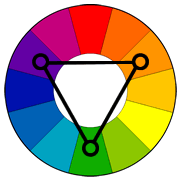
\includegraphics[width=0.2\textwidth]{../png/colors/Triad.png}
        \caption{Barevná paleta aplikace: Trojúhelníkové schema} \label{picture:colors:analog}
    \end{figure}
    \item \emph{Rozděleně-doplňková}: Toto schema vychází z doplňku dvou barev, tedy barev, které jsou v paletě naproti sobě, protější barva je ale rozdělena na dvě. Oproti trojúhelníkovému schematu je méně výrazné, díky čemuž je jednodušší barvy zvolit tak, aby nebyly pro uživatele příliš útočné. Ideální použití je opět jedna základní barva a dvě akcentní.
    \begin{figure}[H]
        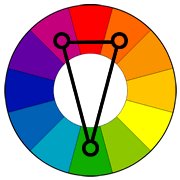
\includegraphics[width=0.2\textwidth]{../png/colors/SplitComplementary.png}
        \caption{Barevná paleta aplikace: Rozděleně-doplňkové schema} \label{picture:colors:splitCom}
    \end{figure}
    \item \emph{Analogová}: Zvolené barvy jsou v barevné paletě přímí sousedé a jedná se tak o \uv{klidné} rozložení, které vytváří jemný design jež je často vidět i v přírodě. Problémem zde může být vhodná volba kontrastu, protože barvy nejsou sami vůči sobě příloš kontrastní a je nutné je od sebe alespoň trochu rozlišit. Ideální použití je jedna dominující barva, druhá doplňková a třetí jako akcentní.
    \begin{figure}[H]
        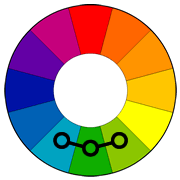
\includegraphics[width=0.2\textwidth]{../png/colors/Analogous.png}
        \caption{Barevná paleta aplikace: Analogové schema} \label{picture:colors:triad}
    \end{figure}
\end{enumerate}

\paragraph{Volba barev pro mou aplikaci.} Jelikož cílem aplikace je pomáhat při práci ve skladu a upozorňovat na důležité zprávy, vyloučil jsem hned ze začátku \emph{analogové} barevné schema, protože jeho barevné rozložení patří spíše na stránky, které jsou pasivnější, nevyžadují tolik interakce s uživatelem a spíše obsah prezentují, než aby vyžadovali jeho zadávání. Zbyly mi tedy velmi podobná rozložení \emph{trojúhelníkové} a \emph{rozděleně-doplňkové}. Podle osobního pocitu jsem vybral základní klidnou barvu: šedozelenou \#009688, a k ní doplňkově-akcentní růžovou \#E91A63 a čistě akcentní tmavě žlutou \#FFC107, jejichž rozložení na barevné paletě je vidět na obrázku \ref{picture:colors:app}. Společně tyto barvy tvoří něco mezi dvěma zvolenými schematy - trojůhelník není ani pravidelný, ani se neblíží k doplňku.\\
\begin{figure}[]
    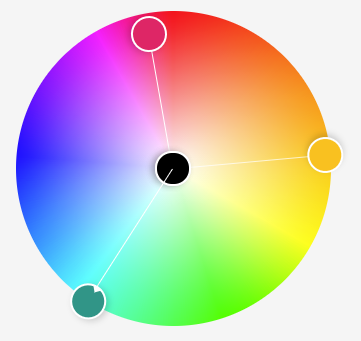
\includegraphics[width=0.4\textwidth]{../png/colors/app.png}
    \caption{Barevná paleta aplikace: Zvolené schema pro mou aplikaci} \label{picture:colors:app}
\end{figure}

\paragraph{Barvy a idempotence akce.} Jelikož mám vybrané dvě akcentní barvy, musel jsem se rohodnout, kde budu kterou z nich používat. Co se týká zobrazování, je vše poměrně jasné: k základní barvě se volně váže doplňkově-akcentní růžová, a čistě akcentní žlutá barva je ponechána pouze pro důležité položky, které je potřeba speciálně zvýraznit. Jiné je to ale u akcí - tlačítek, odkazů apod. Zde jsem se rozhodl barvu tlačítek volit dle idempotence akce, kterou vyvolávají - tedy zda vyvolaná akce způsobuje vedlejší efekty, nebo ji lze vyvolávat stále dokola. Za vedlejší efekty v aplikaci považuji následující situace:
\begin{itemize}
    \item navigace na jinou stránku,
    \item uložení či úprava dat.
\end{itemize}
Naopak akce, které nemají vedlejší efekt jsou všechny ty, které neukládají žádná data ani nemění navigaci, mohou ale měnit aktuální zobrazení stránky, tedy například něco otevřít, skrýt, přesunout, avšak vždy tak, že se jedná o akci pouze na jednom klientu a zůstávají na jedné stránce. Na obrázcích \ref{picture:colors:time_tracker} a \ref{picture:colors:task_fab} je vidět použití jak idempotentních, tak non-idempotentních akcí: tlačítka \emph{storno} a hlavní akční tlačítko pouze skrývají dialog, respektive rozevírají menu, kdežto ostatních tlačítka a volby vždy buďto odesílají data nebo přecházejí na novou stránku.

\begin{figure}[]
    
\includegraphics[width=0.7\textwidth]{../png/app/colors_time_tracker.png}
    \caption{Barvy znázorňující idempotenci akcí: Dialog běžícího času} \label{picture:colors:time_tracker}
\end{figure}
\begin{figure}[]
    
\includegraphics[width=0.3\textwidth]{../png/app/colors_tasks.png}
    \caption{Barvy znázorňující idempotenci akcí: Tlačítko tvorby úkolu} \label{picture:colors:task_fab}
\end{figure}

%%%%%%%%%%%%%%%%%%%%%%%%%%%%%%%%%%%%%%%%%%%%%%%%%%%%%%%%%%%%%%%%%%%%%%%%%%%%%%%%
%%%%%%%%%%%%%%%%%%%%%%%%%%%%%%%%%%%%%%%%%%%%%%%%%%%%%%%%%%%%%%%%%%%%%%%%%%%%%%%%
%%%%%%%%%%%%%%%%%%%%%%%%%%%%%%%%%%%%%%%%%%%%%%%%%%%%%%%%%%%%%%%%%%%%%%%%%%%%%%%%
%%%%%%%%%%%%%%%%%%%%%%%%%%%%%%%%%%%%%%%%%%%%%%%%%%%%%%%%%%%%%%%%%%%%%%%%%%%%%%%%

\section{Záznam stráveného času v úkolech}\label{implementation:time_tracking}

Jedním z požadavků na nový systém byla možnost zaznamenávání stráveného času v úkolech. Jelikož často pracuji v Redmine, což je software pro evidenci požadavků a řízení projektů, kde se čas také zaznamenává, analyzoval jsem, jak se zde se záznamem času pracuje.

\paragraph{Záznam času v Redmine.} V čisté instalaci Redmine je možné čas přidávat k úkolům a nebo celkově k projektům. Zatímco záznam času k projektu se musí provést ze samostatné stránky, záznam času k úkolu je možné spojit s jeho aktualizací. Množství stráveného času ale musí vždy zadat sám uživatel - musí si tedy čas buďto pamatovat, nebo zaznamenávat v další externí aplikaci, či vlastních poznámkách. Jelikož je Redmine open-source, tak existuje hned několik pluginů, které umožňují čas strávený v úkolu stopovat a poté ho zapsat automaticky. Problém, který zde identifikuji já osobně spočívá v tom, že úkolů na Redmine mám často otevřeno i více, nebo naopak žádný, a přesto na některém pracuji například v IDE. Nelze tedy jednoznačně říct, že čas, po který byl úkol otevřen, je stejný jako čas, který byl nad úkolem reálně stráven. Hledal jsem tedy další lepší řešení, a našel vhodnou aplikaci třetí strany.

\paragraph{Záznam času v Toggl.} Toggl je webová aplikace, která nabízí i instalaci nativních agentů pro Windows, Mac a mobilní platofrmy. Díky nainstalovanému agentu je možné spouštět či zastavovat běžící čas klávesovou zkratkou ať už je aktivní browser, IDE, nebo jakýkoliv jiný program. Toto je pro práci, ve které se často přepíná kontext, nebo vznikají pauzy, velmi přínosné. Problém nastává ve chvíli, kdy mám čas uložený v Toggl, ale potřebuji ho zapsat do Redmine. K tomuto účelu jsem napsal vlastní malý doplňěk do Google Chrome, který načte časy uložené v Toggl a otevře záložky s předvyplněnými polemi, ve kterých čas pouze uložím do Redmine. Vše by šlo řešit i zcela automaticky přes API obou služeb, avšak v době psaní tohoto textu ještě není tato synchronizace na dostatečné úrovni a rád mám kontrolu nad tím, které časy vlastně do Redmine zapisuji.

V odstavcích výše jsem se zamyslel nad záznamem času v systému pro řízení obecných projektů. Aplikace pro správu skladu je však přecejen v něčem specifická - jelikož veškerá manipulace se zbožím musí nutně procházet přes ni - všechny položky musí vždy projít čtečkou / být zadány - mělo by být možné stopovat strávený čas přímo v aplikaci

\paragraph{Záznam času v novém skladovém systému.} Pro roli skladníka je poměrně jednoduché automaticky měřit, kolik času strávil v jednotlivých úkolech, a čas odesílat společně s odesláním vyřešení úkolu. U role vedoucího skladu je čas také možné záznamenávat - zde se jedná o přípravu úkolů nebo jejich kontrolou, stále je ale možné práci provádět i mimo tyto obrazovky, například objednávky se mohou zpracovávat mimo systém a pak se pouze jednorázově zadají. Proto jsem také umožnil vedoucímu skladu přidávat strávený čas i ručně.

\paragraph{Pauzování času.} U jakéhokoliv automatického stopování času je nutné mít možnost časomíru pozastavit - typicky například při pauze na oběd či jiné přestávce v práci, během které ale zůstane otevřený jeden úkol. Aplikace vždy zobrazuje, kdy je automatický záznam času spuštěn, a umožňuje ho pozastavit - přičemž u pozastaveného času není možné v úloze provádět žádné akce, až do opětovného spuštění časomíry.

Navrhované řešení automatického záznamu času je samozřejmě možné zcela vypnout v konfiguraci aplikaci, a také ještě bude před ostrým používáním otestováno uživateli. 

%%%%%%%%%%%%%%%%%%%%%%%%%%%%%%%%%%%%%%%%
%%%%%%%%%%%%%%%%%%%%%%%%%%%%%%%%%%%%%%%%

TODO popsat nový vue.config.js a vue ui - dashboard, deps, analyzet atp.

TODO JS Flow

TODO text filtry

https://itnext.io/yes-this-is-how-to-cache-pages-by-url-with-vue-vue-router-and-keep-alive-component-697ed76896e8

TODO kontextové menu

TODO exporty do CSV a JS

TODO renderer tabulek

TODO polyfills https://cli.vuejs.org/guide/browser-compatibility.html

TODO PR do Vuetify?

TODO persistent store

TODO funkční specifikace jednotlivých úkolů?

%%%%%%%%%%%%%%%%%%%%%%%%%%%%%%%%%%%%%%%%
%%%%%%%%%%%%%%%%%%%%%%%%%%%%%%%%%%%%%%%%
%%%%%%%%%%%%%%%%%%%%%%%%%%%%%%%%%%%%%%%%
%%%%%%%%%%%%%%%%%%%%%%%%%%%%%%%%%%%%%%%%

\section{Perličky z vývoje}

\subsection{Špatně importované ikony}

Když jsem byl zhruba v polovině tvorby první použitelné verze aplikace, vyšla aktualizace knihovny \emph{Vuetify}, která z verze 1.x poskočila na verzi 2.0. To ssebou neslo poměrně hodně \emph{breaking changes} \cite{vuetify-2-upgrade}, které jsem ale postupně všechny prošel a aplikaci upravil, takže brzy opět fungovala na nové verzi Vuetify.\\
Po nějakém čase jsem si ale všiml, že u checkboxů a dalších formulářových prvků chybí některé jejich součásti - například u checkboxu to bylo hodně výrazné - tam chyběl celý zaškrtávací čtvereček a byl vidět pouze \emph{label}. Nejprve jsem problém ignoroval s tím, že se pravděpodobně jedná o chybu knihovny, a v některé z dalších verzí bude vše opraveno.\\
Když však ale ani po měsíci nebyly checkboxy stále vidět, začal jsem hledat příčinu problému. Samozřejmě jsem nejprve nahlížel do \emph{Nástrojů vývojáře} v prohlížeči, ale tam jsem nic zajímavého nezjistil - pouze to, že z nějakého důvodu se v mé aplikaci narozdíl od oficiální dokumentace Vuetify \cite{vuetify-doc-checkbox} (kde checkboxy samozřejmě fungovaly), nerenderuje kus HTML, který je má na starost. Založil jsem si tedy nový lokální projekt s Vue.js + Vuetify, kde checkboxy samozřejmě také fungovaly. Postupně jsem tedy začal odebírat různé závislosti z npm, abych přišel na to, která knihovna tento problém způsobuje. Při tomto procesu jsem rovnou zauditoval, zda opravdu potřebuji všechny dříve používané závislosti, a upravil i některé kusy kódu tak, aby závislosti již nebyly potřebné, a tedy jsem kód vlastně zefektivnil a zmenšil velikost výsledné aplikace. Stále jsem ale nemohl přijít na to, proč nefungují checkboxy.\\
Teprve asi po 6 hodinách a asi 40x přeinstalovanými všemi závislostmi, jsem se dostal k importu \emph{Material Design Icons} \cite{mdi}. Vuetify ve verzi 2.0 přidalo do možností své konfigurace klíč, který určuje, který ikonový font se má použit. Při migraci na novou verzi jsem použil ukázkové nastavení této hodnoty, tedy \uv{mdi}. V žádném případě mě totiž nenapadlo, že \emph{Material Design Icons (mdi)} a \emph{Material Icons (md)} není to samé!\\
Po chvilce dalšího ladění s importem ikonek vyšlo najevo, že nastavení \uv{mdi} není kompatibilní s načítáním ikon z CDN Googlu, ale musí se použít balíček z npm. V případě, že chcete načítat ikonky z CDN, musí být hodnota \emph{iconfont} nastavena pouze na \uv{md}. Celý problém, na kterém jsem strávil tolik hodin a nechápavých výrazů šel tedy opravit diffem z ukázky kódu \ref{code:mdi:diff}.

\begin{listing}[h]
\begin{minted}[linenos,frame=lines]{js}
-    iconfont: 'mdi',
+    iconfont: 'md',
\end{minted}
\caption{Diff nastavení fontu ikonek ve Vuetify} \label{code:mdi:diff}
\end{listing}
